% !TEX root = OptimalOffline.tex

Summarising the results of Lemmas \ref{lemma_increasing_power}-\ref{transmission_duration}, the optimal policy $\{\textbf{p},\textbf{s},N\}$ may change transmission powers only at energy arrival epochs i.e. $\forall 1<i<N+1,\ s_i=t_j$ for some $j$. At these epochs, it exhausts the total energy available i.e. $U(s_i)=\ETx(s_i^-)$. The transmission powers are also non-decreasing with time and the optimal policy exhausts the total `receiver time' time allowed, if it does not start transmitting from origin.

Now that we have gained some knowledge regarding the structure of the optimal policy, we consider an example to approach Problem 1. 

Suppose we are given that the receiver can be \textit{on} for a maximum duration of $\TRx_0$. Our goal is to find a transmission policy so that we can minimize the total time at which the transmission of all $B_0$ bits is completed. To do this, we shall first find a feasible solution i.e. one which satisfies all constraints (\ref{pb1_constraint_bits})-(\ref{pb1_constraint_time}) and keep improving upon it, until we have a solution that follows all structural results in Lemma \ref{lemma_increasing_power}-\ref{transmission_duration} (as shown in Theorem \ref{th_algo1_1} later,  these Lemmas form a sufficient condition as well).

We need an initial feasible solution to begin with. For this, we find the minimum energy required by the transmitter so that the transmission can be completed in duration $\TRx_0$ with a constant power. That is, the first $\ETx(t_n)$ such that
\begin{equation}
\TRx_0 g\left(\frac{\ETx(t_n)}{\TRx_0}\right)\geq B_0.
\end{equation}
Let $\widetilde{\TRx}_0\le \TRx_0$ be the time duration such that
\begin{equation}
\widetilde{\TRx}_0 g\left(\frac{\ETx(t_n)}{\widetilde{\TRx}_0}\right)=B_0.
\end{equation}
Let $p_c=\frac{\ETx(t_n)}{\widetilde{\TRx}_0}$. We try to transmit with $p_c$ power starting at time $t=0$. If it does not violate the energy constraint (\ref{pb1_constraint_energy}), we are done with the optimal solution and our transmission is completed in $\widetilde{\TRx}_0<\TRx_0$ time.

If not, we start the transmission at the earliest possible time, such that the transmission with $p_c$ for $\widetilde{\TRx}_0$ time is feasible with respect to (\ref{pb1_constraint_energy}). This transmission policy, will encounter atleast one epoch where total energy consumed till that epoch is equal to the total energy harvested upto it. Let time $t_q$ be the first point where this happens. Let $R$ and $S$ denote the starting and ending time, respectively, of transmission with power $p_c$. Clearly, $S-R=\widetilde{\TRx}_0$. This is shown in Fig. \ref{straight} (a).  Till now we have not argued why we chose such a policy to start with. In fact, Lemma \ref{lemma_Q} shows that this starting solution is a `good' estimate of policy at and before time $t_q$, as both the optimal policy and the above policy run out of all their energy at epoch $t_q$. 

Now, according to Lemma \ref{lemma_energy_consumed}, the optimal policy must finish all available energy when it stops transmission. If transmitting with $p_c$ power does use up all the energy (Fig. \ref{straight} (a)), then we accept the constant power transmission with $p_c$ as our initial policy (line number \ref{init_policy_CP} in Algorithm \ref{init_policy}). If it does not finish up all of $\ETx(t_n)$ with $p_c$ till the end of transmission (shown in Fig. \ref{straight} (b)), we choose a better policy after time $t_q$. Let $\widetilde{B}$ bits be transmitted with power $p_c$ until $S$, which is calculated in line number \ref{init_policy_bits_t_q} of procedure INIT\_POLICY in Algorithm \ref{init_policy}. Now, we require our transmission policy to send $\widetilde{B}$ bits after time $t_q$, in as little time as possible (and of course, before $S$), keeping in mind that the policy should use all $\ETx(t_n)$ amount of energy till it finishes. Algorithm 1 in \cite{Yang} does the job for us. Hence in this case, we choose transmission with $p_c$ till $t_q$ and then the solution of Algorithm 1 in \cite{Yang} after time $t_q$. 

\begin{figure}
\centering
  \centerline{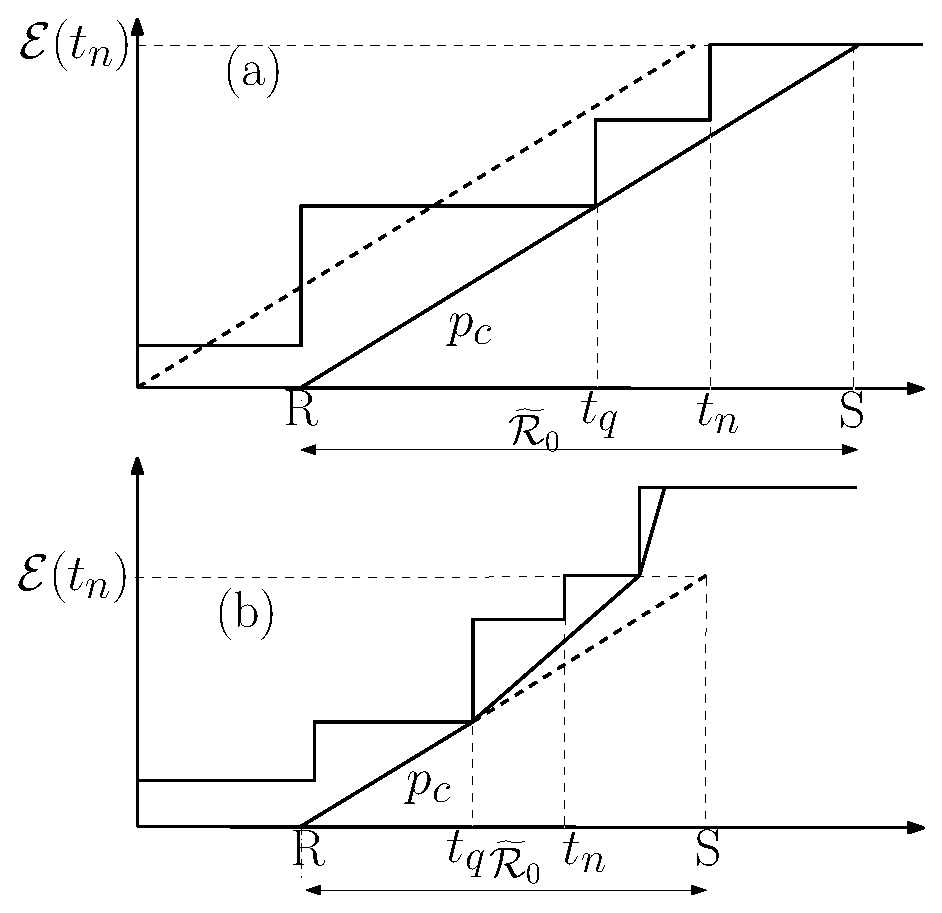
\includegraphics[width=8cm]{straight.eps}}
\caption{Figure showing point $t_q$.}\label{straight}
\end{figure}

\begin{algorithm}
%\algsetup{linenosize=\tiny}
%\alglinenumber{linenosize=\scriptsize}
\caption{Procedure to find initial feasible policy to Problem 1 for Algorithm 2}

\footnotesize%\scriptsize
\label{init_policy}
\begin{algorithmic}[1]
\State \textbf{Initialization}: $B_0$, $\TRx_0$
\Procedure{INIT\_POLICY}{}

\State $n=\displaystyle \argmin_k\left(\left\{t_k | \TRx_0 g\left(\frac{\ETx(t_k)}{\TRx_0}\right)\geq B_0\right\}\right)$ \label{init_policy_Etn}

\State Solve for $\widetilde{T}: \widetilde{T}g\left(\dfrac{\ETx(t_n)}{\widetilde{T}}\right) = B_0$\label{init_policy_CP_time}

\State $p_c=\dfrac{\ETx(n)}{\widetilde{T}}$

\State $q=\displaystyle \argmin_k\ ( \{ t_k | ((\ETx(t_k) - p_ct_k) + p_ct_j) \leq \ETx(t_j),$

$			 						\qquad \qquad \qquad \forall j\in[0,n]  \} )$
\label{init_policy_t_q}
\State $R=t_q-\dfrac{\ETx(t_q)}{p_c}$, $S=t_q+\dfrac{\ETx(t_n)-\ETx(t_q)}{p_c}$

\If {$\ETx(t_n)<\ETx(S^-)$}
	\State $\widetilde{B}=g(p_c)(S-t_q)$\label{init_policy_bits_t_q}  
	\State $\{\textbf{p},\textbf{s},N\}\gets$  Apply Algorithm 1 in \cite{Yang} to 	minimize time of
		\Statex   transmission of $\widetilde{B}$ bits  after time $t_q$ assuming	a  total of $\ETx_{q}$   
		\Statex amount of energy available at $t_q$. 
	\State\Return $\{\{p_c,\textbf{p}\},R,\textbf{s}\},N+1\}$ \label{init_policy_Yang}
	 	\Statex (Transmission with $p_c$ from $R$ to $t_q$ and then with
	 	\Statex policy $\{\textbf{p},\textbf{s},N\}$)
\Else 
	\State\Return $\{\{p_c,p_c\},\{R,t_q,S\},2\}$ \label{init_policy_CP}
\EndIf
\EndProcedure
\end{algorithmic}
\end{algorithm}



\begin{lemma}
In every optimal solution, at energy arrival epoch $t_q$, $U(t_q)=\ETx(t_q^-)$.
\label{lemma_Q}
\end{lemma}
\begin{proof}
We shall prove this by contradiction. First, we make the following claims:

\textbf{Claim 1:} Every optimal transmission policy begins transmission at or before time $R$.

Since, $S-R=\widetilde{\TRx}_0\le \TRx_0$, by Lemma \ref{transmission_duration}, if a transmission policy has to finish before $S$, it has to start before time $\max(S-\TRx_0,0) \le \max(R,0)=R$. 

%Since we are transmitting all the bits at the maximum possible power, no policy that starts after $R$ can finish before $S$. Therefore, any policy that starts after $R$ cannot be optimal.

\textbf{Claim 2:} Every optimal transmission policy ends transmission at or before time $S$.
%This follows immediately from the fact that the policy is optimal.

If it does not, then constant power policy $p_c$ finishing at $S$ will contradict its optimality.
%Let $t_q$ equal to time $t_i$ for some $i\in\mathbb{N}$. 

Suppose we have an optimal transmission policy, say $X$,$\{\bm{p},\bm{s},N\}$, that does not exhaust all its energy at time $t_q$ i.e. $U(t_q)<\ETx(t_q^-)$. Then, by Lemma \ref{lemma_energy_consumed}, it does not change its transmission power at $t_q$. Let the transmission power of $X$ be $p_{j-1}$ at $t_q$ and $p_{j-1}$ starts from $s_{j-1}$ and goes till $s_j$. Now, $s_j<S$ by \textit{Claim 2}. Further, power $p_c$ exhausts all energy by $t_q$. So,
\begin{align}
&p_c(t_q-R)=\ETx(t_q^-)\label{eqlemmaQ1}.
\end{align}
But, by constraint (\ref{pb1_constraint_energy}),
\begin{align}
&p_c(t_q-R)+p_c(s_j-t_q)\le \ETx(s_j^-),
\\
& p_c(s_j-t_q)\stackrel{(\ref{eqlemmaQ1})}{\le} \ETx(s_j^-)-\ETx(t_q^-),
\\
& p_c(s_j-t_q)< \ETx(s_j^-)-U(t_q)=p_{j-1}(s_j-t_q),
\\
& p_c<p_{j-1} .\label{eqlemmaQ2}
\end{align}
If ${j-1}= 1$, then power at $t_q$ is the first transmission power $p_1$. But then by \eqref{eqlemmaQ2}, $p_1 > p_c$. By the definition of $p_c$, we must have $s_{1} > R$, but this will contradict \textit{Claim 1}.

So ${j-1}\ge 2$, which means that the power of transmission must change at least once between $R$ and $t_q$. By Lemma \ref{lemma_energy_consumed}, $X$ has used all energy by $s_{j-1}$ and $s_{j}$ as well. So, $p_{j}(\ETx(s_{j}^-)-\ETx(s_{j-1}^-))$ is the maximum energy available between time $s_{j-1}$ and $s_{j}$. If $R<s_{j-1}$, then $p_c$ (by \eqref{eqlemmaQ2}) uses more energy, than available between $s_{j-1}$ and $s_{j}$, which is not possible. If $s_{j-1}\le R$ then $p_{j-1}$ uses more than maximum energy available (given by $p_c(t_q-R)=\ETx(t_q^-)$ ) between time $R$ and $t_q$, violating energy constraint \eqref{pb1_constraint_energy}. 

Therefore, every optimal transmission policy must use all energy till epoch $t_q$. 

%If the optimal policy does have a power higher than $p_c$ at $t_q$, then it must have the same power of transmission either from some epoch, say $t_k$, or from the beginning of transmission. If $t_k>R$, we can show that $p_c$ becomes infeasible with respect to energy constraint (\ref{pb1_constraint_energy}) at $t_k$. If $t_k<R$, $p$ becomes infeasible with energy constraint \eqref{pb1_constraint_energy} at time $R$. Now, only thing left is the optimal policy begins transmission with power $p$. If so, then it has to begin transmission after time $R$ which follows from equation (\ref{eqlemmaQ2}). This violates \textit{Claim 1}. Therefore every optimal transmission policy must use all energy till epoch $t_q$.
\end{proof}

Now that we have an initial feasible solution, we shall proceed to improve upon this policy as follows. The formal algorithm is presented as Algorithm \ref{Algorithm1}. We explain the procedure by an example. Assume that the starting feasible solution is given by the constant power policy, as shown by dotted line in Fig. \ref{figure_example_Algorithm1} (a), where $t_q=t_2$. We first assign the following initial values for the initial feasible policy - transmission power left of $t_2$ as $p_l=p_c$, power right of $t_2$ as $p_r=p_c$, start time $T_{start}=R$, stop time $T_{stop}=S$, epoch at which $p_l$ ends as $t_l=t_2$, epoch at which $p_r$ starts as $t_r=t_2$. Now, we increase $p_r$, keeping $t_r$ fixed, till it reaches $p_r'$ which hits epoch $t_3$, as shown by the solid line in Fig \ref{figure_example_Algorithm1} (a). As in total we need to transmit $B_0$ bits, the decrease in bits transferred by $p_r$ to $p_r'$ (RHS of \eqref{eq_example1}) is compensated by calculating appropriate $p_l'$ according to the following equation, where LHS represents the increase in bits transmitted from $p_l$ to $p_l'$.
\begin{align}
&g(p_l')\frac{\ETx(t_l^-)}{p_l'}-g(p_l)(t_l-T_{start})=-g(p_r)(T_{stop}-t_r)\nonumber\\
&+g(p_r')(\mathcal{P}(t_r,t_3))\frac{\ETx(T_{stop}^-)-ETx(t_r^-)}{\mathcal{P}(t_r,t_3)}.
\label{eq_example1}
\end{align}   
Having got a feasible $p_l'$, as shown in Fig. \ref{figure_example_Algorithm1} (a), we assign $T_{start}'$ with the point where $p_l'$ starts, $T_{stop}'$ with the point where $p_r'$ ends. $t_r'$ gets the value $t_3$ and $t_l'$ remains same as $t_l=t_2$. Note that parameters $\{T_{start}',T_{stop}',t_l',t_r',p_l',p_r'\}$ define the policy at the end of first iteration. 

In the next iteration, the portion of transmission between $t_l'=t_2$ to $t_r'=t_3$ is not updated. In this iteration, we try to increase $p_r'$ about $t_r'$ till it hits the feasibility equation \eqref{pb1_constraint_energy} of energy. $p_r'$ could virtually be increased to infinity. But transmission with infinite power for 0 time does not transmit any bits. So we assign $t_r''=t_2$ and $p_r''=\mathcal{P}(t_2,t_3)$. With this change in $p_r'$ to $p_r''$, we again calculate $p_l''$ which compensates the decrease in bits transferred after $t_r'$. But the calculated $p_l''$ becomes infeasible at $t_1$ as shown in Fig. \ref{figure_example_Algorithm1} (b). Hence, we set $p_l''$ to the maximum feasible power $\mathcal{P}(t_1,t_2)$ as shown in Fig. \ref{figure_example_Algorithm1} (c). With this $p_l''$, we re-calculate $p_r''$, so as to transmit $B_0$ bits in total. $t_l''$ is assigned to $t_1$, $t_r''$ remains $t_3$. $T_{start}''$ and $T_{stop}''$ as calculated to values marked in Fig. \ref{figure_example_Algorithm1} (c). The final policy at the end of second iteration is shown by solid line in Fig. \ref{figure_example_Algorithm1} (c). Like this, we continue to the third iteration, by improving the policy (to finish earlier) before $t_l''$ and after $t_r''$ and so on.


\begin{figure}
\centering
  \centerline{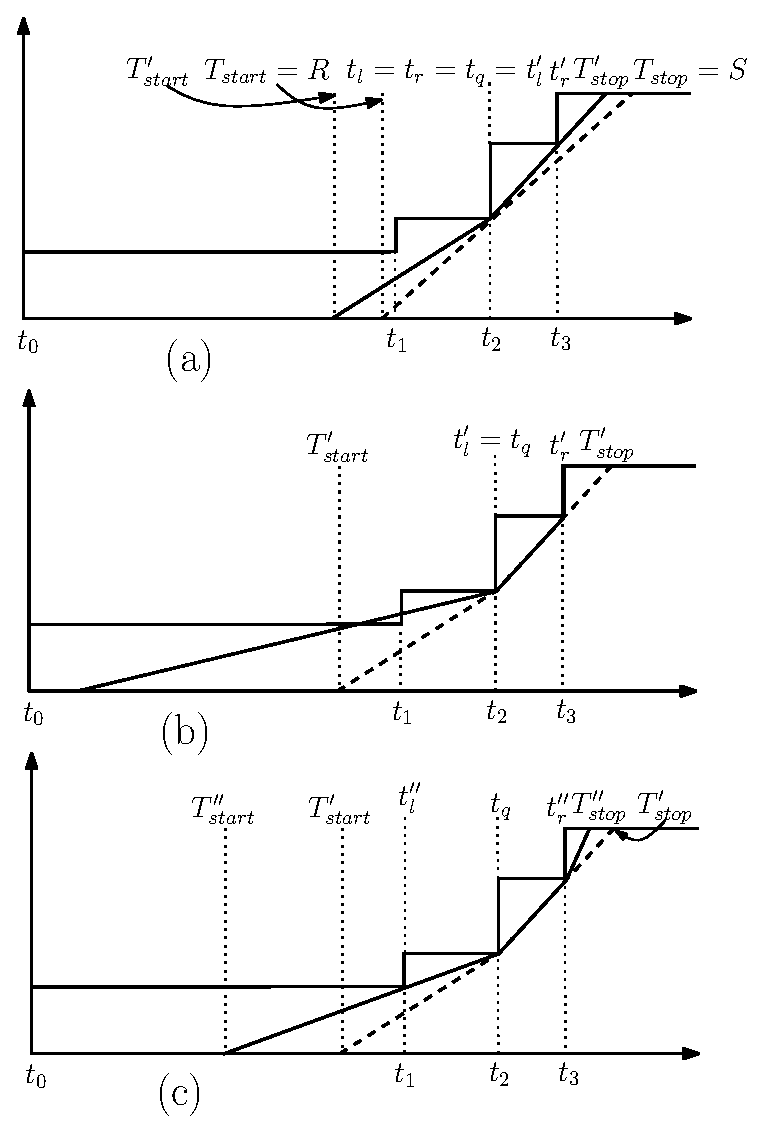
\includegraphics[width=8cm]{example_algo1.eps}}
\caption{Figures showing (a) first  and (c) second iteration of the Algorithm \ref{Algorithm1} through an example. (b) representes an intermidiate step in second iteration. In any diagram, the dashed line represent previous iteration policy and solid line is the present iteration policy.}\label{figure_example_Algorithm1}
\end{figure}


Now we describe the algorithm in steps. In any iteration, let $t_{l}$ and $t_{r}$ be the first and last energy arrival epochs where the power of transmission changes. $p_l$ and $p_r$ are the transmission power before $t_l$ and after $t_r$ respectively. $T_{start}$ and $T_{stop}$ are the start and finish time of the policy, found in any iteration. The policy found by the Algorithm in-between time $t_l$ and $t_r$ is stored in array \textbf{p} and \textbf{s}. The possible cases that can happen in an iteration of the Algorithm are shown in Fig. \ref{figure_Algorithm1}. 

Step1: The Algorithm tries to increase $p_r$ as much as possible till it hits the boundary of energy constraint \eqref{pb1_constraint_energy} as shown in Fig. \ref{figure_Algorithm1}(a). Then the Algorithm calculates the possible power $p_l'$ such that it transmits same number of bits in total with the previous iteration policy, i.e. $B_0$, as shown in line number \ref{algo_bits_left_1} and \ref{algo_bits_left_2} of Algorithm \ref{Algorithm1}. 

Step2: If $p_l'$ is feasible, which is the case shown in Fig. \ref{figure_Algorithm1}(a), the policy changes $p_l$ to $p_l'$ and $p_r$ to $p_r'$ (with $t_r$ to $t_r'$). $T_{start}$ and $T_{stop}$ are changed accordingly to start and end points of $p_l'$  and $p_r'$. 

Step3: If $p_l'$ is not feasible, as shown in Fig. \ref{figure_Algorithm1}(b), then $p_l'$ is set to be the maximum possible feasible power from $t_l$, as shown in Fig. \ref{figure_Algorithm1}(c). Now, $p_r'$ is calculated so as to settle the transmission of equal number of bits as the previous iteration. 
%We can be sure that $p_r'$ calculated now, would not be infeasible. 
In this case $t_l$ gets updated to $t_l'$.  

Going back to the first step of the algorithm where we were increasing $p_r$, it could happen, as shown in Fig. \ref{figure_Algorithm1}(d), that $p_r$ can increase to infinity without violating the energy constraint \eqref{pb1_constraint_energy}. This happens when there is no energy epoch between $t_r$ and $T_{stop}$. In this scenario, transmission is stopped at $t_r$,i.e. $T_{stop}$ gets updated to $t_r$ and both $t_r$ and $p_r$ are set to the last values in array \textbf{s},\textbf{p} receptively. This is shown in Fig. \ref{figure_Algorithm1}(d). Now, the Algorithm proceeds to calculate $p_l'$ as done in Step1, and continues as before to check whether $p_l'$ is feasible and decides according to Step2 or Step3.

\begin{figure}
\centering
  \centerline{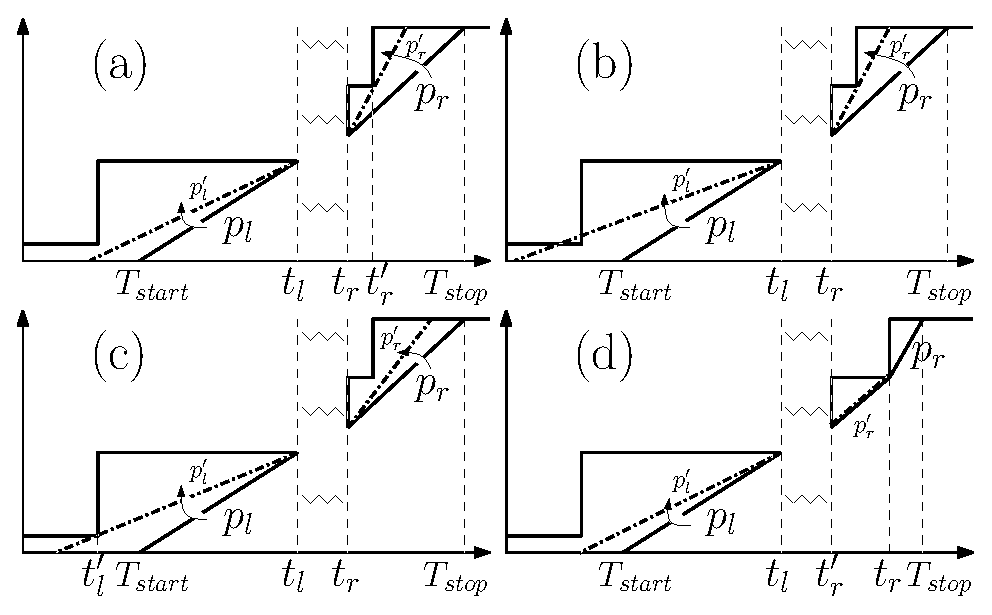
\includegraphics[width=8cm]{Algorithm1.eps}}
\caption{Figures showing any iteration of the Algorithm \ref{Algorithm1}. The solid line represents the transmission policy in the previous iteration. The dash dotted lines in (a), (b), (c), (d) represent the possible configurations of policy in the current iteration.}\label{figure_Algorithm1}
\end{figure}

This is how the algorithm proceeds to generate a new transmission policy in every iteration, which begins and ends earlier than the policy given by the previous iteration, until a point is reached where either $T_{stop}-T_{start}>\TRx_0$ or $T_{start}=0$. Suppose the Algorithm terminates with $T_{start}=0$ and $T_{start}-T_{stop}\le\TRx_0$, then the policy at this iteration is the optimal policy, as will be proved in Theorem \ref{th_algo1_2}. 


For the case where the algorithm terminates with $T_{stop}-T_{start}>\TRx_0$, let $\{T_{start}',T_{stop}',p_l',p_r',t_l',t_r'\}$ be the values in the termination iteration and $\{T_{start},T_{stop},p_l,p_r,t_l,t_r$ be the values in the previous iteration. Then, the possible valid configurations can be one of the three shown in Fig. \ref{figure_Algorithm1} (a) (c) (d). Note that $\ETx(T_{stop}^-)=\ETx(T_{stop}'^-)$ in all the cases. (In case Fig. \ref{figure_Algorithm1} (d) we can assume that $T_{stop}'=t_r^+$ and transmission exists after $t_r$, but with infinite power. Since transmitting with infinite power for $0$ time does not transmit any bits, we would transmit the same number of bits, as we did prior to this modification). Thus, by Lemma \ref{lemma_increase_time}, we can verify that $(T_{stop}'-T_{start}')>(T_{stop}-T_{start})$. Since $(T_{stop}'-T_{start}')>\TRx_0>(T_{stop}-T_{start})$, there must exist a solution to equation presented in line number \ref{algo_solve_eqn} of Algorithm \ref{Algorithm1}. Let the policy obtained from the solution start and end at $T_{start}''$ and $T_{stop}''$. Then $T_{stop}''$ and $T_{start}''$ would lie in-between $T_{stop}$,$T_{stop}'$ and $T_{start}$,$T_{start}'$ respectively. Also, $T_{stop}''-T_{start}''=\TRx_0$.

So we can conclude by stating that, the solution to Algorithm \ref{Algorithm1} satisfies Lemma \ref{transmission_duration}. Now, according to the definition of $t_n$ and $t_q$ in line number \ref{init_policy_Etn} and \ref{init_policy_t_q} of INIT\_POLICY, $t_q\le t_n$ and $\ETx(t_q)<\ETx(t_n)$. Since $t_n$ is defined as the first energy arrival epoch by which $B_0$ bits can be transmitted in $\TRx_0$ time, any transmission policy which ends at or before $t_n$ should take more than $\TRx_0$ time to transmit all of $B_0$ bits. As $t_q\le t_n$, we are guaranteed that no transmission policy can finish at or before $t_q$. Hence in the iterations of the algorithm $t_r$ can never decrease beyond $t_q$. As $t_q$ is present in the initial solution, $t_q$ always exists in the final solution to Algorithm \ref{Algorithm1}.   
